\DocumentMetadata{pdfversion=2.0, pdfstandard=A-4}
\documentclass[aspectratio=1610]{beamer} % for presentation on TV
\usetheme{madrid}
\usecolortheme{RIT}

\usepackage{bookmark}
\usepackage{booktabs}
\usepackage{cite}
\usepackage{gensymb}
\usepackage{graphicx}
\usepackage{xcolor,colorspace}
\usepackage{tikz}
\usepackage[]{circuitikz}
\usepackage{environ}
\makeatletter
\newsavebox{\measure@tikzpicture}
\NewEnviron{scaletikzpicturetowidth}[1]{%
  \def\tikz@width{#1}%
  \def\tikzscale{1}\begin{lrbox}{\measure@tikzpicture}%
  \BODY
  \end{lrbox}%
  \pgfmathparse{#1/\wd\measure@tikzpicture}%
  \edef\tikzscale{\pgfmathresult}%
  \BODY
}
\makeatother
\usepackage{pgfplots}
\usepackage{pgfplotstable}
\pgfplotsset{compat = newest}
\pgfplotsset{
  every axis legend/.append style =
    {
      cells = { anchor = east },
      draw  = none
    }
}
\pgfplotsset{
  myplot/.style =
    {
      cycle list name = color list , 
      every x tick label/.append style  =
        { 
          /pgf/number format/.cd ,
           precision = 1 , 
           fixed         ,
           zerofill
        },
      xlabel = \(V_{CC}~(V)\),
      ylabel = \(V_{ref}~(V)\),
    },
}
\makeatletter
\pgfplotsset{ % Tufte-like plot
  tufte axes/.style =
    {
      after end axis/.code =
        {
          \draw ({rel axis cs:0,0} -| {axis cs:\pgfplots@data@xmin,0})
            -- ({rel axis cs:0,0}  -| {axis cs:\pgfplots@data@xmax,0});
          \draw ({rel axis cs:0,0} |- {axis cs:0,\pgfplots@data@ymin})
            -- ({rel axis cs:0,0}  |-{axis cs:0,\pgfplots@data@ymax});
        },
      axis line style = {draw = none},
      tick align      = outside,
      tick pos        = left
    }
}
\makeatother

\usepackage{amsmath}
\usepackage{mathtools} % loads amsmath and fixes its bugs, empheq, etc
\usepackage{amssymb}
\usepackage{sympytex}
\usepackage{siunitx}
\sisetup{detect-all=true}   % ensure proper font weight
\sisetup{per-mode = repeated-symbol}    % ensure "/" unit delineator
\sisetup{range-phrase = --,range-units = brackets} % hyphenated ranges, SI syntax
\DeclareMathSymbol{\varOmega}{\mathalpha}{operators}{"0A}   % upright omega for ohms
\providecommand*{\Ohm}{\varOmega}   % for siunitx
\DeclareSIUnit\sq{\ensuremath{\Box}}    % sheet resistance
\DeclareSIUnit{\Siemens}{S}
\DeclareSIUnit{\torr}{Torr} % add torr to siunitix 3
\DeclareSIUnit\sig{\ensuremath{\sigma}}
\DeclareSIUnit\ppm{ppm}
\usepackage{xfrac}

% *** SUBFIGURE PACKAGES ***
\usepackage[caption=false,font=footnotesize]{subfig}

\usepackage{stfloats}

\usepackage{fontspec}
\setmainfont{STIXTwoText}[
	Extension		= .otf,
	UprightFont		= *-Regular,
	BoldFont		= *-Bold.otf,
	ItalicFont		= *-MediumItalic.otf,
	BoldItalicFont 	= *-BoldItalic.otf
]
\usepackage[math-style=ISO]{unicode-math}
\setmathfont{STIXTwoMath-Regular.otf} % for symbols
\usepackage{microtype}
\UseMicrotypeSet[protrusion]{basicmath} % disable protrusion for tt fonts
\urlstyle{same}
\newcommand{\unifrac}[2]{\mbox{% making sure we don't get a line break
    {\addfontfeatures{RawFeature=+numr}#1}%
    ⁄% That slash is U+2044 FRACTION SLASH, which has special spacing
    {\addfontfeatures{RawFeature=+dnom}#2}%
    }}
\usepackage{semidevsymbRommel}
\usepackage{filecontents}
\usepackage{feynmf} % For drawing Feynman squiggly arrows (photons)
% % % % % % % % % % % % % % % % % % % % % % % % % % % % % % % % % % % % % % %
\usetikzlibrary{arrows, decorations.markings,shapes, positioning} 
\tikzstyle arrowstyle=[scale=1]
%% Local defines: %%
% define bra/ket:
\def\bra#1{\left<#1\right|}
\def\ket#1{\left|#1\right>}
\newcommand{\tendsto}[1]{%
	\xrightarrow{\smash{\raisebox{-2ex}{$\scriptstyle#1$}}}}

\graphicspath{{images/}{drawings/}}

\usepackage{orcidlink}
\RequirePackage[type={CC},modifier={by-nc-nd},version={4.0},lang={english}]{doclicense}

\usepackage{datetime2} % to satisfy the "\today" in \hypersetup
\DTMusemodule{english}{en-US}
\usepackage{hyperref}
\hypersetup{
    colorlinks=true,
	bookmarksnumbered,
    bookmarksopen=true,
    linkcolor=rit-orange,
    filecolor=magenta,      
    urlcolor=cyan,
%%%%%%%%%%%%%%%% METADATA %%%%%%%%%%%%%%%%%%%%	
    pdftitle={EE726 Midterm},
	pdfsubject={Banba et al. Sub-1-V CMOS Bandgap Reference},
    pdfauthor={Chris Biancone},
	pdfpublisher={Chris Biancone},
	pdfkeywords={bandgap, voltage reference},
%%%%%%%%%%%%%%%%%%%%%%%%%%%%%%%%%%%%%%%%%%%%%%
	pdfproducer=luaLaTeX-1.17.0,
	pdfdate=\today,
	pdflang={en},pdfmetalang={en},
	pdflicenseurl={},
    pdfpagemode=FullScreen,
}
\usepackage[nameinlink,capitalize]{cleveref}

% correct bad hyphenation here
\hyphenation{op-tical net-works semi-conduc-tor}

\usefonttheme{serif}

\title[Banba Bandgap]{\bfseries Review of Sub-1-V Bandgap Reference}
\author[C. Biancone]{Chris Biancone}
\date[]\today{}
\institute[RIT]{EE726 Mixed-Signal IC Design \\ Electrical and Microelectronic Engineering \\ Rochester Institute of Technology}

\begin{document}

    \setbeamertemplate{itemize item}[square]
	\setbeamertemplate{itemize subitem}[square]
	\setbeamertemplate{itemize subsubitem}[circle]
	\setbeamertemplate{enumerate items}[default]
	\setbeamertemplate{enumerate subitems}[default]
    \logo{\includegraphics[height=0.75cm]{RIT_KGCOE1.eps}\vspace{238pt}}
    \setbeamertemplate{frametitle}{\color{rit-brown}\bfseries\insertframetitle\par\normalsize\insertframesubtitle\par\vspace{-4pt}\color{rit-orange}\hrulefill}
    \setbeamercovered{transparent=0}
	\setbeamertemplate{caption}[numbered]


\begin{frame}
	\titlepage
\end{frame}

\begin{frame}{Voltage References}
    \begin{itemize}
        \item Extremely important:
        \begin{itemize}
            \item Bias circuits, signal conditioning, power regulation, VCO \dots
        \end{itemize}
        \item After the 1950s, Zener diodes began to replace the Weston standard cell~\cite{Weston1893,Zener1934}
        \begin{itemize}
            \item Miniaturized, but reduced lifetime~\cite{Baker1960}
        \end{itemize}
        \item Manufacturing advancements led to highly-doped pn junctions, reducing their temperature dependence~\cite{Hibiber1964}
        \item The bandgap reference circuit leverages additional device properties to render the output voltage a function of only the material bandgap
    \end{itemize}

    \begin{columns}[T]
        \column{0.45\textwidth}
        \begin{figure}
            \centering
            \includegraphics[height=0.3\textheight]{images/standardcell.png}
            \label{fig:standardcell}
        \end{figure}
        \column{0.45\textwidth}
        \begin{figure}
            \centering
            \includegraphics[height=0.3\textheight]{images/zener.png}
            \label{fig:zener}
        \end{figure}
    \end{columns}
    \vfill
\end{frame}

\begin{frame}{Basic Bandgap Theory}{PN Junction}

\begin{columns}[c]
	\column{0.45\textwidth}
    \begin{itemize}
        \item Current is related to \(V_f\), which is linearly dependent on temperature
        \item The saturation current can be shown by approximating the temperature dependence of \(n_i\)~\cite{Brugler1967}
        \item Normally, PN junctions don't behave this way due to surface effects \& depeletion region generation / recombination~\cite{Sah1957}
        \item This \emph{does} nicely describe the workings of a BJT
    \end{itemize}

	\column{0.55\textwidth}
    \small
	\begin{align}
        V_T &= \frac{kT}{q} \approx \qty{8.617e-5}{\V\per\K} \label{eq:vt} \\
        I &= I_s\left[\exp{\left(\frac{V_f}{V_T}\right)} - 1\right] \label{eq:pn_i}
    \end{align}
    \begin{align}
        {n_i}^2 &= C_0 T^3 \exp{\left(\frac{-E_G}{kT}\right)} \nonumber \\
        I_s &\simeq C_{p^+n,n^+p} T^{\beta_{p,n}} \exp{\left(\frac{-E_G}{kT}\right)} \label{eq:pn_is}
    \end{align}
\end{columns}
\end{frame}

\begin{frame}{Basic Bandgap Theory}{BJT}

    \begin{columns}[T]
        \column{0.45\textwidth}
        \begin{itemize}
            \item Performing a Taylor series expansion on the formula for \(V_{BE}\) as a function of \(I_C\) yields this mess:
        \end{itemize}
        \column{0.55\textwidth}
    \end{columns}
    \tiny
    \begin{gather}
        \hspace*{-12pt}
        V_{BE} = \frac{kT_0}{q} \Biggl\{ \ln{\biggl(\frac{I_C}{I_s T_0}\biggr)} + \Biggl[\ln{\biggl(\frac{I_C}{I_s T_0}\biggr)} - \biggl( \beta + \frac{E_{G_0}}{kT_0} \biggr) \Biggr] \biggl( \frac{T}{T_0} - 1 \biggr) \nonumber - \frac{\beta}{2} \biggl( \frac{T}{T_0} - 1 \biggr)^2 + \cdots + \frac{\beta (-1)^{(n-1)}}{n(n-1)} \biggl( \frac{T}{T_0} - 1 \biggr)^n + \cdots \Biggr\}\label{eq:pn_taylor} \\
        V_{BE} > 4V_T,\qquad T < 2T_0 \nonumber
    \end{gather}
    \vspace{-4pt}
    \begin{columns}[c]
        \column{0.45\textwidth}
        \normalsize
        \begin{itemize}
            \item[] which neatly shows that as doping concentration increases, temperature dependence decreases~\cite{Sah1962}
            \item It is possible to choose a ratio of devices \(\Theta\) to compensate this thermal relationship
        \end{itemize}
        \column{0.55\textwidth}
        \normalsize
        \begin{equation}
            \Theta = r\ln\biggl(\frac{I_{C_2}}{I_{S_2}T_0}\biggr) - m\ln\biggl(\frac{I_{C_1}}{I_{S_1}T_0}\biggr)\label{eq:ratio}
        \end{equation}
    \end{columns}
    \end{frame}

\begin{frame}{Basic Bandgap Theory}{Thermal Compensation}

        \begin{columns}[c]
            \column{0.45\textwidth}
            \begin{itemize}
                \item By properly selecting \(\Theta\), the first order temperature dependence of current density is eliminated
                \item Since \(E_{G_0}\) is much greater than \(\Phi V_{T_0}\), \(V_{ref}\) becomes primarily a function of the bandgap
                \item In a standard bandgap core, the temperature coefficient of \(V_{BE} = \qty{-2}{\mV\per\degree\C}\) is cancelled by the \(\Delta V_{BE}\) from the current density ratio~\cite{Widlar1967,Pease1990}
            \end{itemize}
        
            \column{0.55\textwidth}
            \small
            \begin{gather}
                \Delta V_{BE} = V_T \ln{\Biggl(\frac{I_{C_2}}{I_{C_1}}\Biggr)}, \quad I_C = I_{C_0}\biggl(\frac{T}{T_0}\biggr) \nonumber \\
                \Delta V_{BE} = V_T \ln{\biggl(\frac{T_0}{T}\biggr)} \label{eq:d_vbe}
            \end{gather}
        \end{columns}
\end{frame}

\begin{frame}{Basic Bandgap Theory}{Limitations}

    \begin{columns}[c]
        \column{0.45\textwidth}
        \begin{itemize}
            \item Many designs like those of Widlar, Kuijk, and Brokaw enhance the performance with additional error amplification and series regulation
            \item With \(E_{G_{Si}} = \qty{1.12}{\eV}\), standard bandgap topologies have a lower limit around \qty{1.25}{\V}, dependent on the threshold voltage of the devices used for its construction
        \end{itemize}
        \vspace*{-4pt}
        \small
        \begin{equation}
            V_{ref} = V_{f_1} + \frac{R_2}{R_3}V_T\ln\Biggl(\frac{R_2}{R_1}N\Biggr)
        \label{eq:conv_vout}
        \end{equation}
    
        \column{0.55\textwidth}
        \small
        \begin{figure}[!t]
            \centering
            \begin{scaletikzpicturetowidth}{0.65\columnwidth}
            \begin{circuitikz}[american,scale=\tikzscale,transform shape]
                \ctikzset{tripoles/mos style/arrows}
                \ctikzset{tripoles/pmos style/nocircle}
                \ctikzset{resistors/scale=0.75}
                \ctikzset{diodes/scale=0.75}
                \ctikzset{voltage=raised}
                \ctikzset{voltage/shift=4}
                \ctikzset{legacy transistors text}
                \draw (0,-0.5) node[op amp,scale=0.5] (opamp1) {};
                \draw (-0.75,-0.25) node[circ] (in1) {} node[left] {$V_a$};
                \draw (-0.75,-0.75) node[circ] (in2) {} node[left] {$V_b$};
                \draw (in1) -- (opamp1.-);
                \draw (in2) -- (opamp1.+);
                \draw (1.5,-0.5) node[pmos](M1){M1};
                \draw (M1.S) node[vdd]{$V_{CC}$} (1.5,1.0);
                \draw (M1.G) to[short] (opamp1.out);
                \draw (M1.D) -- (1.5,-1.5) to[R,l=$R_1$,v=$\biggl(\frac{R_2}{R_3}\biggr)dV_f$,f>^=$I_1$] (1.5,-4.0) -- (1.5,-6) to[D,l=$D_1$,v=$V_{f_1}$] (1.5,-7.5) node[ground]{} (1.5,-8);
                \draw (2,-4) node[circ] (in1) {} node[right] {$V_a$} -* (1.5,-4);
                \draw (4,-1.5) to[R,l=$R_2$,v=$\biggl(\frac{R_2}{R_3}\biggr)dV_f$,f>^=$I_2$] (4,-4.0) to[R,l=$R_3$,v=$dV_f$] (4,-6) to[D,v=$V_{f_2}$] (4,-7.5) node[ground]{} (4,-8);
                \draw (4.5,-4) node[circ] (in1) {} node[right] {$V_b$} -* (4,-4);
                \draw (4.75,-6) to[D] (4.75,-7.5) node[ground]{} (4.75,-8);
                \path (5,-6.75) -- node{\huge$\dots$} (6,-6.75);
                \draw (6.25,-6) to[D,l=$N\cdot D_2$] (6.25,-7.5) node[ground]{} (6.25,-8);
                \draw (6.25,-6) -- (4,-6);
                \draw (1.5,-1.5) -- (6.25,-1.5) node[ocirc](vref){} node[right]{$V_{ref}$};
            \end{circuitikz}
            \end{scaletikzpicturetowidth}
            \caption{Conventional bandgap reference circuit schematic used for comparison. Redrawn from~\cite{Banba1999}.}\label{fig:conv_bg}
            \end{figure}
    \end{columns}
\end{frame}

\begin{frame}{Banba et al. Design}{}
    \normalsize
    \begin{columns}[c]
        \column{0.45\textwidth}
        \begin{itemize}
            \item Presented at 1998 Symposium on VLSI Circuits
            \item Current-mode operation
            \item Resistive dividers placed in parallel with diode devices
            \item Additional current sources used in a current-mirror configuration
            \item Desired equilibrium: \(I_1 = I_2 = I_3\)
        \end{itemize}
    
        \column{0.55\textwidth}
        \small
        \begin{figure}[!t]
            \centering
            \begin{scaletikzpicturetowidth}{\columnwidth}
            \begin{circuitikz}[american,scale=\tikzscale,transform shape]
                \ctikzset{tripoles/mos style/arrows}
                \ctikzset{tripoles/pmos style/nocircle}
                \ctikzset{resistors/scale=0.75}
                \ctikzset{diodes/scale=0.75}
                \ctikzset{voltage=raised}
                \ctikzset{voltage/shift=1}
                \ctikzset{legacy transistors text}
                \draw (0,0) node[op amp,scale=0.5] (opamp1) {};
                \draw (-0.75,0.25) node[circ] (in1) {} node[left] {$V_a$};
                \draw (-0.75,-0.25) node[circ] (in2) {} node[left] {$V_b$};
                \draw (in1) -- (opamp1.-);
                \draw (in2) -- (opamp1.+);
                \draw (1.5,0) node[pmos](M1){M1};
                \draw (M1.S) node[vdd]{$V_{CC}$} (1.5,1.0);
                \draw (M1.D) -- (1.5,-1.0) -- (1.5,-3) to[D,l=$D_1$,v=$V_{f_1}$,i>^=$I_{1a}$] (1.5,-4.5) node[ground]{} (1.5,-5);
                \draw (4,0) node[pmos](M2){M2};
                \draw (M2.S) node[vdd]{$V_{CC}$} (4,1.5);
                \draw (M2.D) --(4,-1);
                \draw (9,0) node[pmos](M3){M3};
                \draw (M3.S) node[vdd]{$V_{CC}$} (4,1.0);
                \draw (M3.D) --(9,-1);
                \draw (M3.G) to[short] (opamp1.out);
                \draw (2,-1) node[circ] (in1) {} node[right] {$V_a$} -* (0,-1);
                \draw (4,-1) to[R,l=$R_3$,v=$dV_f$,i>^=$I_{2a}$] (4,-3) to[D,v=$V_{f_2}$] (4,-4.5) node[ground]{} (4,-5);
                \draw (7.75,-1) node[circ] (in1) {} node[right] {$V_b$} -* (4,-1);
                \draw (4.75,-3) to[D] (4.75,-4.5) node[ground]{} (4.75,-5);
                \path (5,-3.75) -- node{\huge$\dots$} (6,-3.75);
                \draw (6.25,-3) to[D,l=$ND_2$] (6.25,-4.5) node[ground]{} (6.25,-5);
                \draw (6.25,-3) -- (4,-3);
                \draw (7.5,-1) -- (7.5,-2) to[R,l_=$R_2$,i>_=$I_{2b}$] (7.5,-4) -- (7.5,-4.5) node[ground]{} (7.5,-5);
                \draw (0,-1) -- (0,-2) to[R,l=$R_1$,i>^=$I_{1b}$] (0,-4) -- (0,-4.5) node[ground]{} (0,-5);
                \draw (9,-1) -- (9,-2) to[R,l=$R_4$,i>_=$I_{3}$] (9,-4) -- (9,-4.5) node[ground]{} (9,-5);
                \draw (10,-1) node[ocirc] (vref) {} node[right] {$V_{ref}$} -* (9,-1);
            \end{circuitikz}
            \end{scaletikzpicturetowidth}
            \caption{Proposed bandgap reference circuit schematic. Redrawn from~\cite{Banba1999}.}\label{fig:prop_bg}
            \end{figure}
    \end{columns}
\end{frame}

\begin{frame}{Banba et al. Design}{}
    \normalsize
    \begin{columns}[c]
        \column{0.45\textwidth}
        \begin{itemize}
            \item All else equal, lower \(V_{ref}\) limit is reduced by a factor of \(\sfrac{R2}{R4}\)
            \item With \(M_{1,2,3}\) in saturation \(V_{CC}\) can theoretically be lowered to \(V_{f}\) if \(V_{ref} < V_f\) 
        \end{itemize}
        \small
        \begin{gather}
            V_{ref,old} = V_{f_1} + \frac{R_2}{R_3}V_T\ln\Biggl(\frac{R_2}{R_1}N\Biggr)\nonumber\\
            V_{ref,new} = \frac{R_4}{R_2}V_{f_1} + \frac{R_4}{R_3}V_T \ln{(N)}
        \end{gather}
    
        \column{0.55\textwidth}
        \small
        \begin{figure}[!t]
            \centering
            \begin{scaletikzpicturetowidth}{\columnwidth}
            \begin{circuitikz}[american,scale=\tikzscale,transform shape]
                \ctikzset{tripoles/mos style/arrows}
                \ctikzset{tripoles/pmos style/nocircle}
                \ctikzset{resistors/scale=0.75}
                \ctikzset{diodes/scale=0.75}
                \ctikzset{voltage=raised}
                \ctikzset{voltage/shift=1}
                \ctikzset{legacy transistors text}
                \draw (0,0) node[op amp,scale=0.5] (opamp1) {};
                \draw (-0.75,0.25) node[circ] (in1) {} node[left] {$V_a$};
                \draw (-0.75,-0.25) node[circ] (in2) {} node[left] {$V_b$};
                \draw (in1) -- (opamp1.-);
                \draw (in2) -- (opamp1.+);
                \draw (1.5,0) node[pmos](M1){M1};
                \draw (M1.S) node[vdd]{$V_{CC}$} (1.5,1.0);
                \draw (M1.D) -- (1.5,-1.0) -- (1.5,-3) to[D,l=$D_1$,v=$V_{f_1}$,i>^=$I_{1a}$] (1.5,-4.5) node[ground]{} (1.5,-5);
                \draw (4,0) node[pmos](M2){M2};
                \draw (M2.S) node[vdd]{$V_{CC}$} (4,1.5);
                \draw (M2.D) --(4,-1);
                \draw (9,0) node[pmos](M3){M3};
                \draw (M3.S) node[vdd]{$V_{CC}$} (4,1.0);
                \draw (M3.D) --(9,-1);
                \draw (M3.G) to[short] (opamp1.out);
                \draw (2,-1) node[circ] (in1) {} node[right] {$V_a$} -* (0,-1);
                \draw (4,-1) to[R,l=$R_3$,v=$dV_f$,i>^=$I_{2a}$] (4,-3) to[D,v=$V_{f_2}$] (4,-4.5) node[ground]{} (4,-5);
                \draw (7.75,-1) node[circ] (in1) {} node[right] {$V_b$} -* (4,-1);
                \draw (4.75,-3) to[D] (4.75,-4.5) node[ground]{} (4.75,-5);
                \path (5,-3.75) -- node{\huge$\dots$} (6,-3.75);
                \draw (6.25,-3) to[D,l=$ND_2$] (6.25,-4.5) node[ground]{} (6.25,-5);
                \draw (6.25,-3) -- (4,-3);
                \draw (7.5,-1) -- (7.5,-2) to[R,l_=$R_2$,i>_=$I_{2b}$] (7.5,-4) -- (7.5,-4.5) node[ground]{} (7.5,-5);
                \draw (0,-1) -- (0,-2) to[R,l=$R_1$,i>^=$I_{1b}$] (0,-4) -- (0,-4.5) node[ground]{} (0,-5);
                \draw (9,-1) -- (9,-2) to[R,l=$R_4$,i>_=$I_{3}$] (9,-4) -- (9,-4.5) node[ground]{} (9,-5);
                \draw (10,-1) node[ocirc] (vref) {} node[right] {$V_{ref}$} -* (9,-1);
            \end{circuitikz}
            \end{scaletikzpicturetowidth}
            \end{figure}
    \end{columns}
\end{frame}

\normalsize

\begin{frame}{Their Results}{}

    \centering{They did not manage to achieve operation under \qty{1}{\V} \(V_{CC}\)!}
    \begin{columns}[c]
        \column{0.5\textwidth}
        \begin{figure}
            \includegraphics[height=0.6\columnwidth]{banba_fig_3.png}
            \caption{What they expected.}\label{fig:banba_expected}
        \end{figure}
    
        \column{0.5\textwidth}
        \begin{figure}
            \includegraphics[height=0.55\columnwidth]{banba_fig_7.png}
            \caption{What they got.}\label{fig:banba_measured}
        \end{figure}
    \end{columns}
    \end{frame}

\begin{frame}{Their Results}{What Happened?}

    \begin{columns}[c]
        \column{0.45\textwidth}
        \begin{itemize}
            \item Authors worked at Toshiba
            \item A \qty{400}{\nm} flash memory process was selected with very high threshold voltages
            \item This prevented their design from even turning on before \qty{1}{\V} \(V_{CC}\), which they claimed operation under
            \item Native NMOS devices were used at the inputs of the op-amp to compensate for the poor threshold voltages
            \item Why this choice of fabrication process?
        \end{itemize}
    
        \column{0.55\textwidth}
        \begin{table}[]
            \centering
            \begin{tabular}{c|c}
            \toprule
                Simulation Process & Unknown Parameters \\
            \midrule
                \(V_{th_p}\) & \qty{-0.3}{\V} \\
                \(V_{th_n}\) & \qty{0.4}{\V} \\
            \bottomrule
            \end{tabular}
            \caption{Simulated threshold voltages.}
            \label{tab:sim_th}
        \end{table}
        \begin{table}[]
            \centering
            \begin{tabular}{c|c}
            \toprule
                Flash Memory & \qty{0.4}{\um} P-sub CMOS \\
                Process &  1 poly, 1 silicide, 2 metal \\
            \midrule
                \(V_{th_p}\) & \qty{-1.0}{\V} \\
                \(V_{th_n}\) & \qty{0.7}{\V} \\
                \(V_{th_n,nat}\) & \qty{-0.2}{\V} \\
            \bottomrule
            \end{tabular}
            \caption{Fabricated threshold voltages.}
            \label{tab:fab_th}
        \end{table}
    \end{columns}
\end{frame}

\begin{frame}{Their Results}{Significance}

    \begin{columns}[c]
        \column{0.45\textwidth}
        \begin{itemize}
            \item Papers have collectively been cited over 800 times
            \item Obvious impact on the industry despite poor hardware results
            \item PSRR was not reported
            \item In reporting distributions, the conventional design had 34 data points, whereas the new design only had 23
            \item Process parameters for the BJT devices may also have been useful
        \end{itemize}
    
        \column{0.55\textwidth}
        \begin{figure}
            \includegraphics[height=0.4\columnwidth]{hmm.png}            
        \end{figure}
    \end{columns}
\end{frame}

\begin{frame}{Recommendations}{}

    \begin{columns}[c]
        \column{0.45\textwidth}
        \begin{itemize}
            \item Verify performance in a process designed for low voltage operation
            \item Use same number of data points for design comparison
            \item Low-tempco thin film resistors, trimmed resistors \& BJTs~\cite{Brokaw1974,Malcovati2001,Mok2004}
            \item Substitute resistors with MOS devices~\cite{Buck2002}
        \end{itemize}
    
        \column{0.55\textwidth}
        \begin{figure}
            \includegraphics[width=0.8\columnwidth]{no_resistors.png}
            \caption{Schematic of resistorless bandgap circuit proposed in~\cite{Buck2002}.}
        \end{figure}
    \end{columns}
\end{frame}

\begin{frame}{Recent Developments}{}

    \begin{columns}[c]
        \column{0.45\textwidth}
        \begin{itemize}
            \item A group from the University of Pisa proposed a design in 2021 for supply volages down to \qty{0.5}~\cite{Ria2021}
            \item Uses a ``classic'' all-CMOS bandgap core modified with low threshold and native devices in a \qty{0.18}{\um} process
            \item Combined with a switched-cap integrator for offset cancellation and low-frequency noise reduction
            \item \(V_{ref} = \qty{220}{\mV}\) with sensitivity of \qty{45}{\ppm\per\degree\C} with current draw of \qty{630}{\nA}
            \item Considerable performance analysis shown in the paper
        \end{itemize}
    
        \column{0.55\textwidth}
        \begin{figure}
            \includegraphics[width=0.7\columnwidth]{oops_all_cmos.png}
            \caption{Schematic of all-CMOS design proposed in~\cite{Ria2021}.}
        \end{figure}
    \end{columns}
\end{frame}

\begin{frame}{A Generic Approach}{}

    \begin{columns}[c]
        \column{0.45\textwidth}
        \begin{itemize}
            \item Banba's design was constructed in the C\=adence gpdk45\_v5.0 to see its performance in a process that was designed for low voltage operation
            \item Its performance was compared with the stated conventional design, using the same device parameters
            \item All \qty{1}{\V}-LVT devices were used
        \end{itemize}
        \begin{table}[]
            \centering
            \begin{tabular}{c|c}
            \toprule
                gpdk45\_v5.0 & \qty{45}{\nm} \\
                & 1 s, 1 p, 11 m \\
            \midrule
                \(V_{th_p}\) & \qty{-0.34}{\V} \\
                \(V_{th_n}\) & \qty{0.28}{\V} \\
            \bottomrule
            \end{tabular}
            \caption{\qty{1}{\V}-LVT threshold voltages, around the sizes simulated.}
            \label{tab:sim_th}
        \end{table}
    
        \column{0.55\textwidth}
        \begin{figure}
            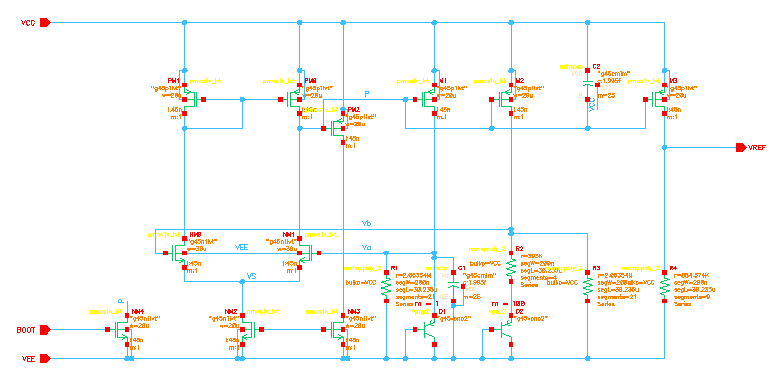
\includegraphics[width=\columnwidth]{bg_prop.eps}
            \caption{Schematic of the new bandgap as simulated in C\=adence Virtuoso.}\label{fig:gpdk_prop}
        \end{figure}
    \end{columns}
\end{frame}

\begin{frame}{It Works!}{}

    \begin{columns}[c]
        \column{0.45\textwidth}
        \begin{itemize}
            \item Operation down to about \qty{0.7}{\V} was achieved for both designs
            \item Shows the devere dependence on the threshold voltage
            \item Proposed design is able to achieve much lower \(V_{ref}\) and lower temperature variation
            \item Startup behavior for the proposed design was consistently slower
            \item Often showed less stability in operating range
            \begin{itemize}
                \item Could be due to lack of optimization and poor startup circuit implementation
            \end{itemize}
        \end{itemize}

        \column{0.55\textwidth}
        \begin{figure}[!t]
            \centering
            \pgfplotstableread[col sep=comma,]{data/bandgap.csv}\datatable
            \begin{tikzpicture}
                \begin{axis}[
                    myplot,
                    tufte axes,
                    every axis legend/.append style = {at={(0.9,0.5)}}]
        
                    \addplot table [x expr = \thisrowno{0},
                            y expr = \thisrowno{3}]{\datatable};
                    \addlegendentry{Proposed}
                    \addplot table [x expr = \thisrowno{0},
                            y expr = \thisrowno{1}]{\datatable};
                    \addlegendentry{Conventional}
                \end{axis}
            \end{tikzpicture}
            \vspace{-6pt}
            \caption{\(V_{CC}\) sweep results.}\label{fig:gpdk_bandgap_results}
        \end{figure}
    \end{columns}
\end{frame}

\begin{frame}[allowframebreaks]
    \frametitle{References}
    \small
    \bibliographystyle{IEEEtranDOI}
    \bibliography{main.bib}
    \small
\end{frame}

\end{document}